\section{Validierung}
In diesem Kapitel geht es darum, Anforderungen und Eigenschaften des Aktor- und Sensorbausteins zu testen.
\subsection{Sensorbaustein}
\subsubsection{ESD Test}
Der Sensorbaustein wird wie eine Unterputzsteckdose verbaut und die Frontplatte dient als User-Interface. 
Genauer bedeutet es, dass der Benutzer, die Touchflächen der Frontplatte berühren muss, um mit dem Sensorbaustein zu interagieren. 
Durch das berühren kann es jedoch zu elektrostatischen Entladungen kommen, die der Sensorbaustein überstehen muss.
Deswegen wurde mithilfe eines ESD-Tests, getestet bis zu welchem Prüfschärfegrad, also bis zur welcher Entladespannung der Sensorbaustein funktioniert.
In der Tabelle \ref{tab: ESD_Testablauf} sind die Prüfschärfegrade und deren Spannungen abgebildet.
Für den Test wurde die Kontaktentladung genommen, mit welcher eine Entladung über einen Finger nachgestellt wird.\\
Der Testablauf war wie folgt \cite{schleuniger_emv_w8_2020}:\\
\\
- Beginn beim tiefsten Schärfegrad\\
- 1 Entladung/s\\
- mind. 10 Entladungen, jeweils auf jeder Touchfläche\\


\begin{figure}[H]
	\centering
	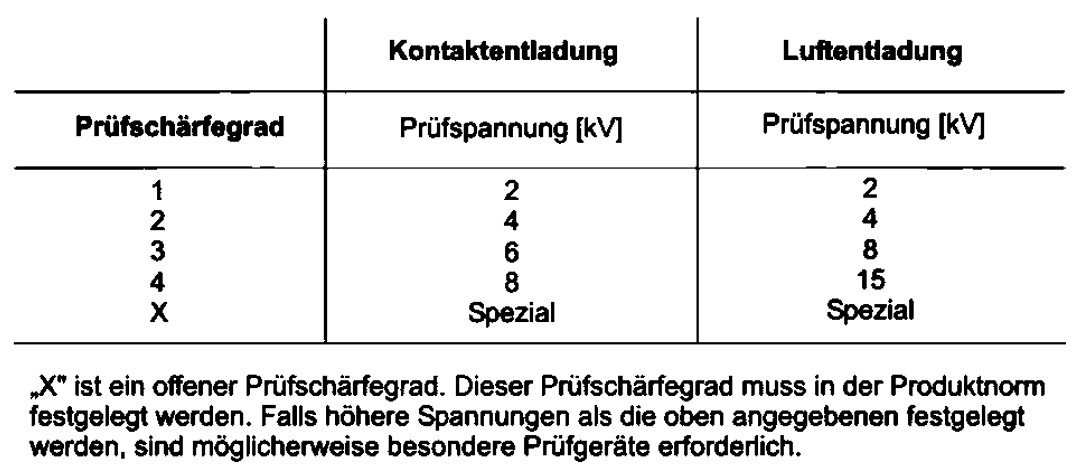
\includegraphics[width=0.8\textwidth]{graphics/ESD_Testablauf.jpg}
	\caption{ESD Testablauf \cite{schleuniger_emv_w8_2020}}
	\label{tab: ESD_Testablauf}
\end{figure}

Das Resultat war, dass der Sensorbaustein beim Prüfschärfegrad 4 Schaden nahm. Bei geringeren Spannungen war er funktionstüchtig. Was bedeutet, dass der Sensorbaustein Prüfschärfegrad 3 mit 6\,kV erreicht hat. Der Schaden beim Grad 4 war sichtbar und befand sich beim Seriell/UART-Wandler (Abbildung: \ref{pic: ESD_Schaden}), was nicht zu erwarten war. Der betroffene Pin war die Spannungsversorgung des IC's, dazu wurden direkt die 5\,V der Eingangsspeisung genommen, die Entweder über USB oder Pins angeschlossen wird. Beide Spannungsversorgungen sind miteinander verbunden, da in der Anwendung nur eines von beidem verwendet wird. Theoretisch wäre es auch möglich gewesen die 3.3\,V als Versorgung des Seriell/UART-Wandlers zu nehmen, die Frage ist, ob dann der gleiche Schaden aufgetreten wäre. Die Schutzdioden welche Über- und Unterspannung ableiten sind mit Ground bzw. 3.3\,V verbunden und nur der Seriell/UART-Wandler und der DC/DC Wandler sind an der 5\,V Speisung angeschlossen. Schlussendlich ist der Strom über den Seriell/UART-Wandler abgeflossen und hat ihn zerstört.

\subsubsection{Energieverbrauch}
\begin{figure}[H]
	\centering
	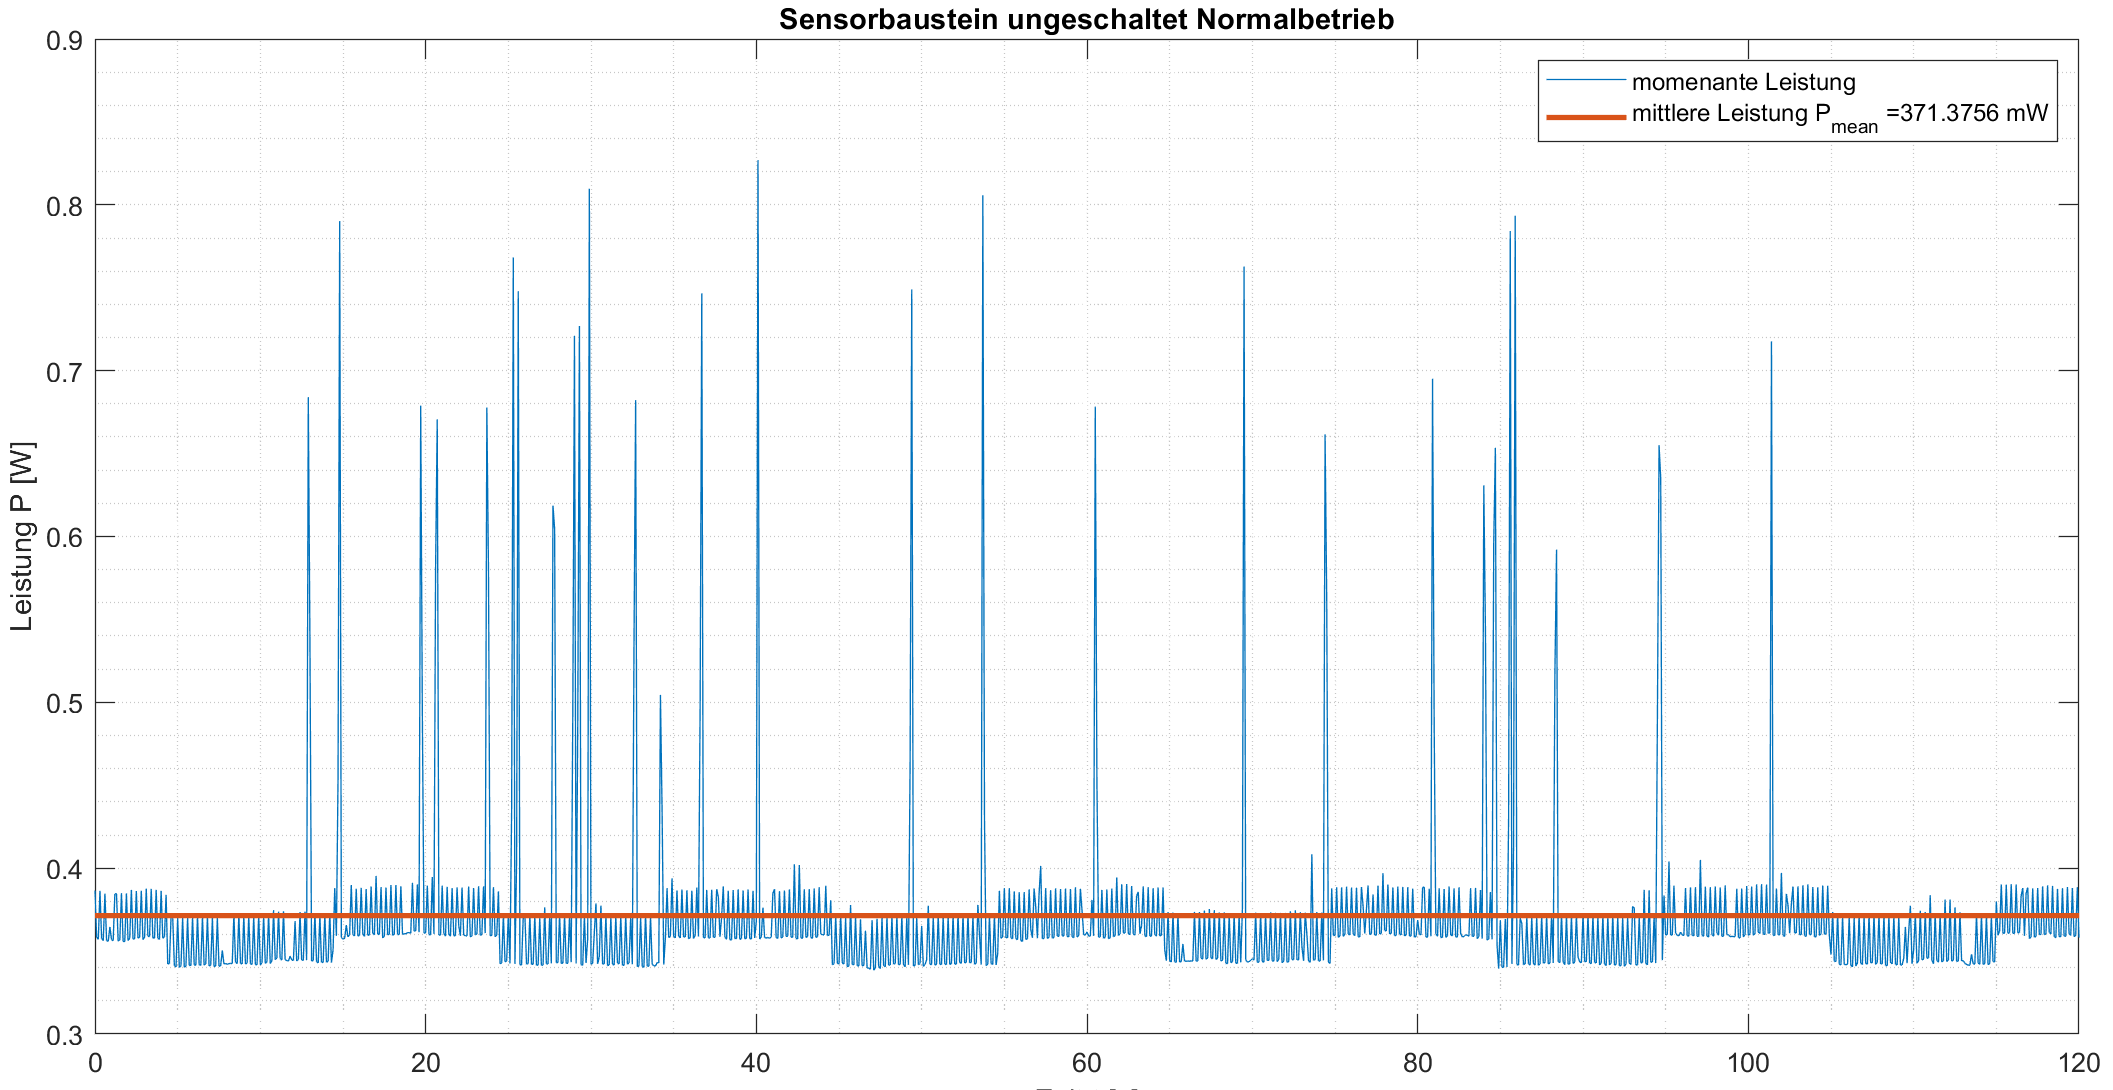
\includegraphics[width=1\textwidth]{graphics/Sensorbaustein_ungeschaltet.png}
	\caption{Die Leistung des Sensorbausteins, wenn er nicht bedient wird und mit dem Netzwerk verbunden ist}
	\label{pic: Sensorbaustein_ungeschaltet}
\end{figure}

\begin{figure}[H]
	\centering
	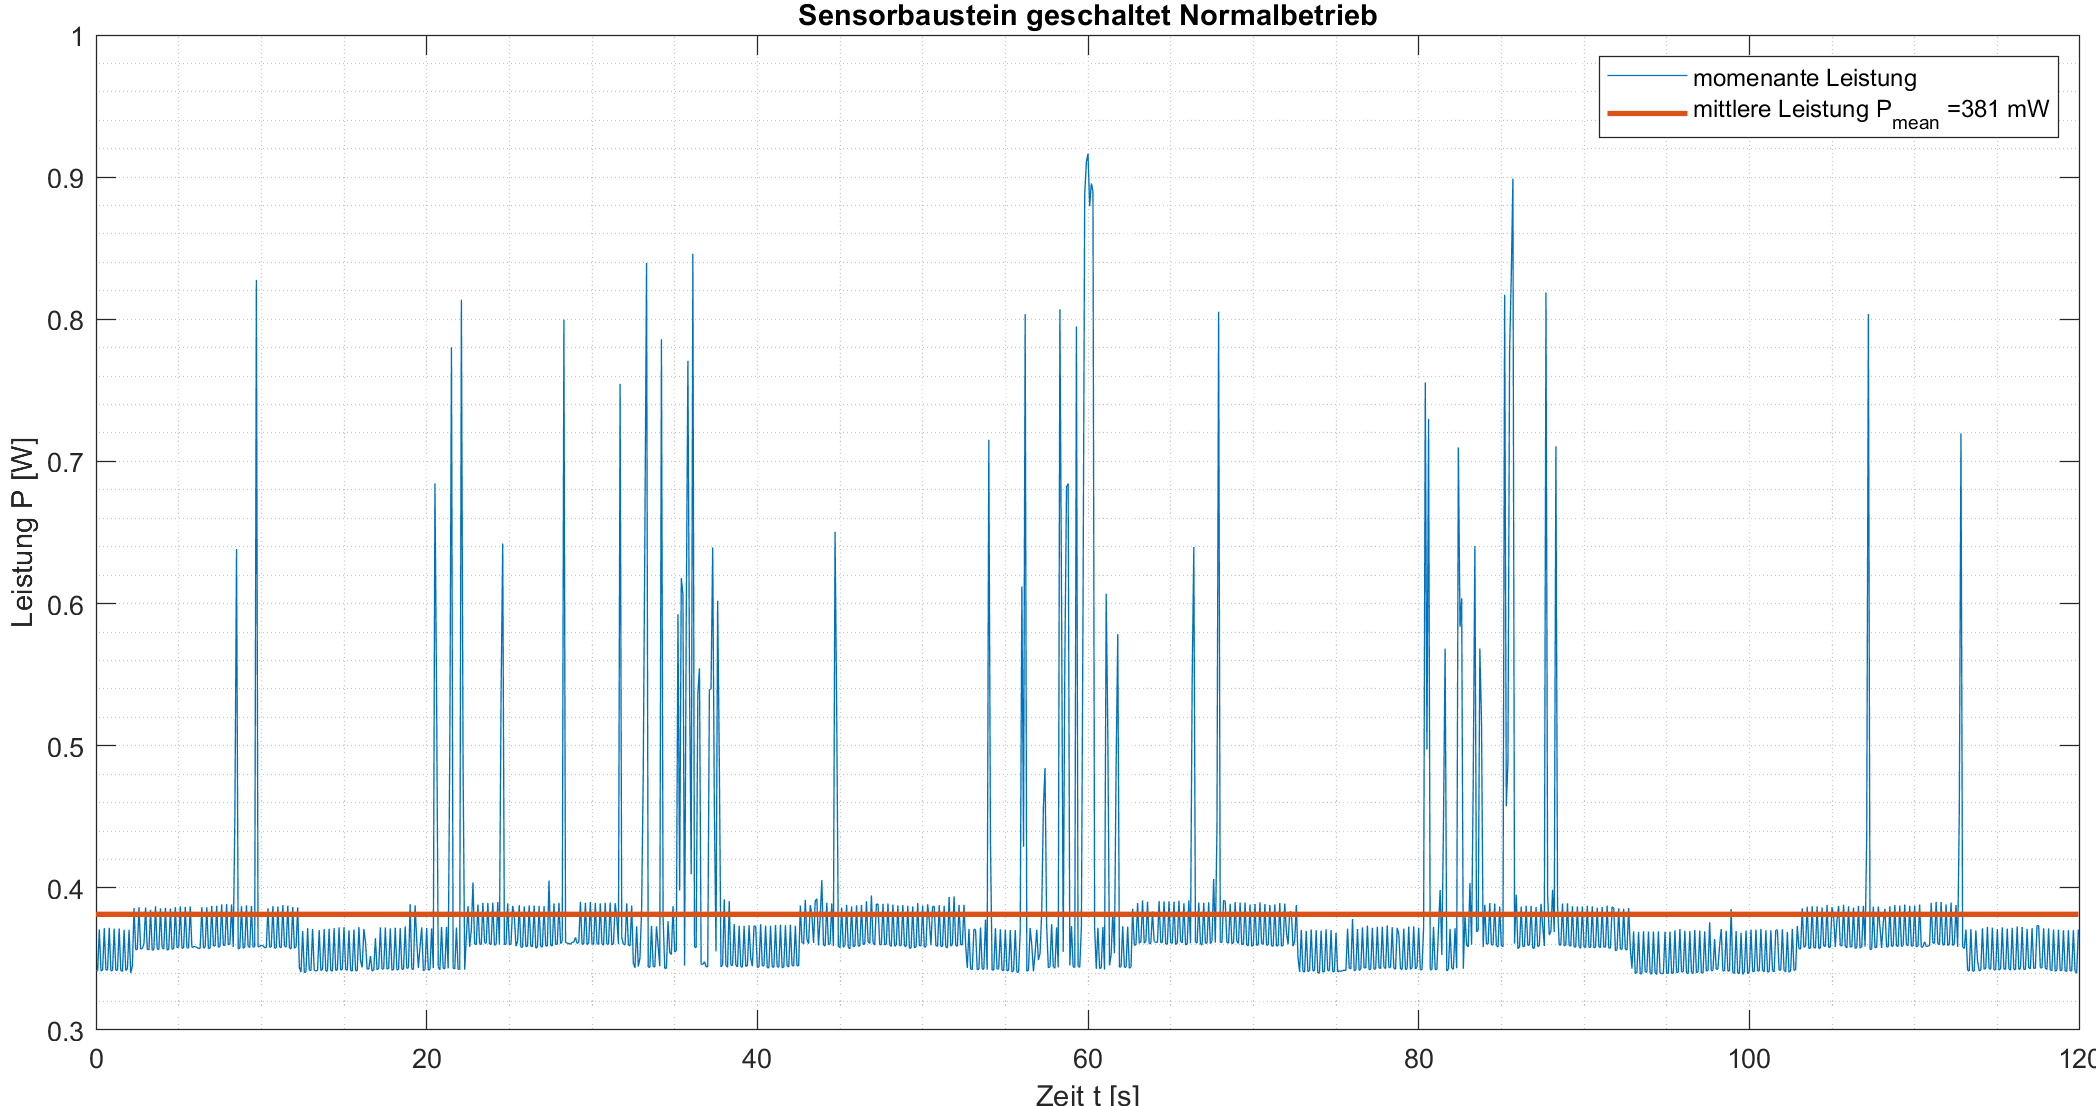
\includegraphics[width=1\textwidth]{graphics/Sensorbaustein_geschaltet.png}
	\caption{Die Leistung des Sensorbausteins, wenn er bedient wird und mit dem Netzwerk verbunden ist}
	\label{pic: Sensorbaustein_geschaltet}
\end{figure}

\begin{figure}[H]
	\centering
	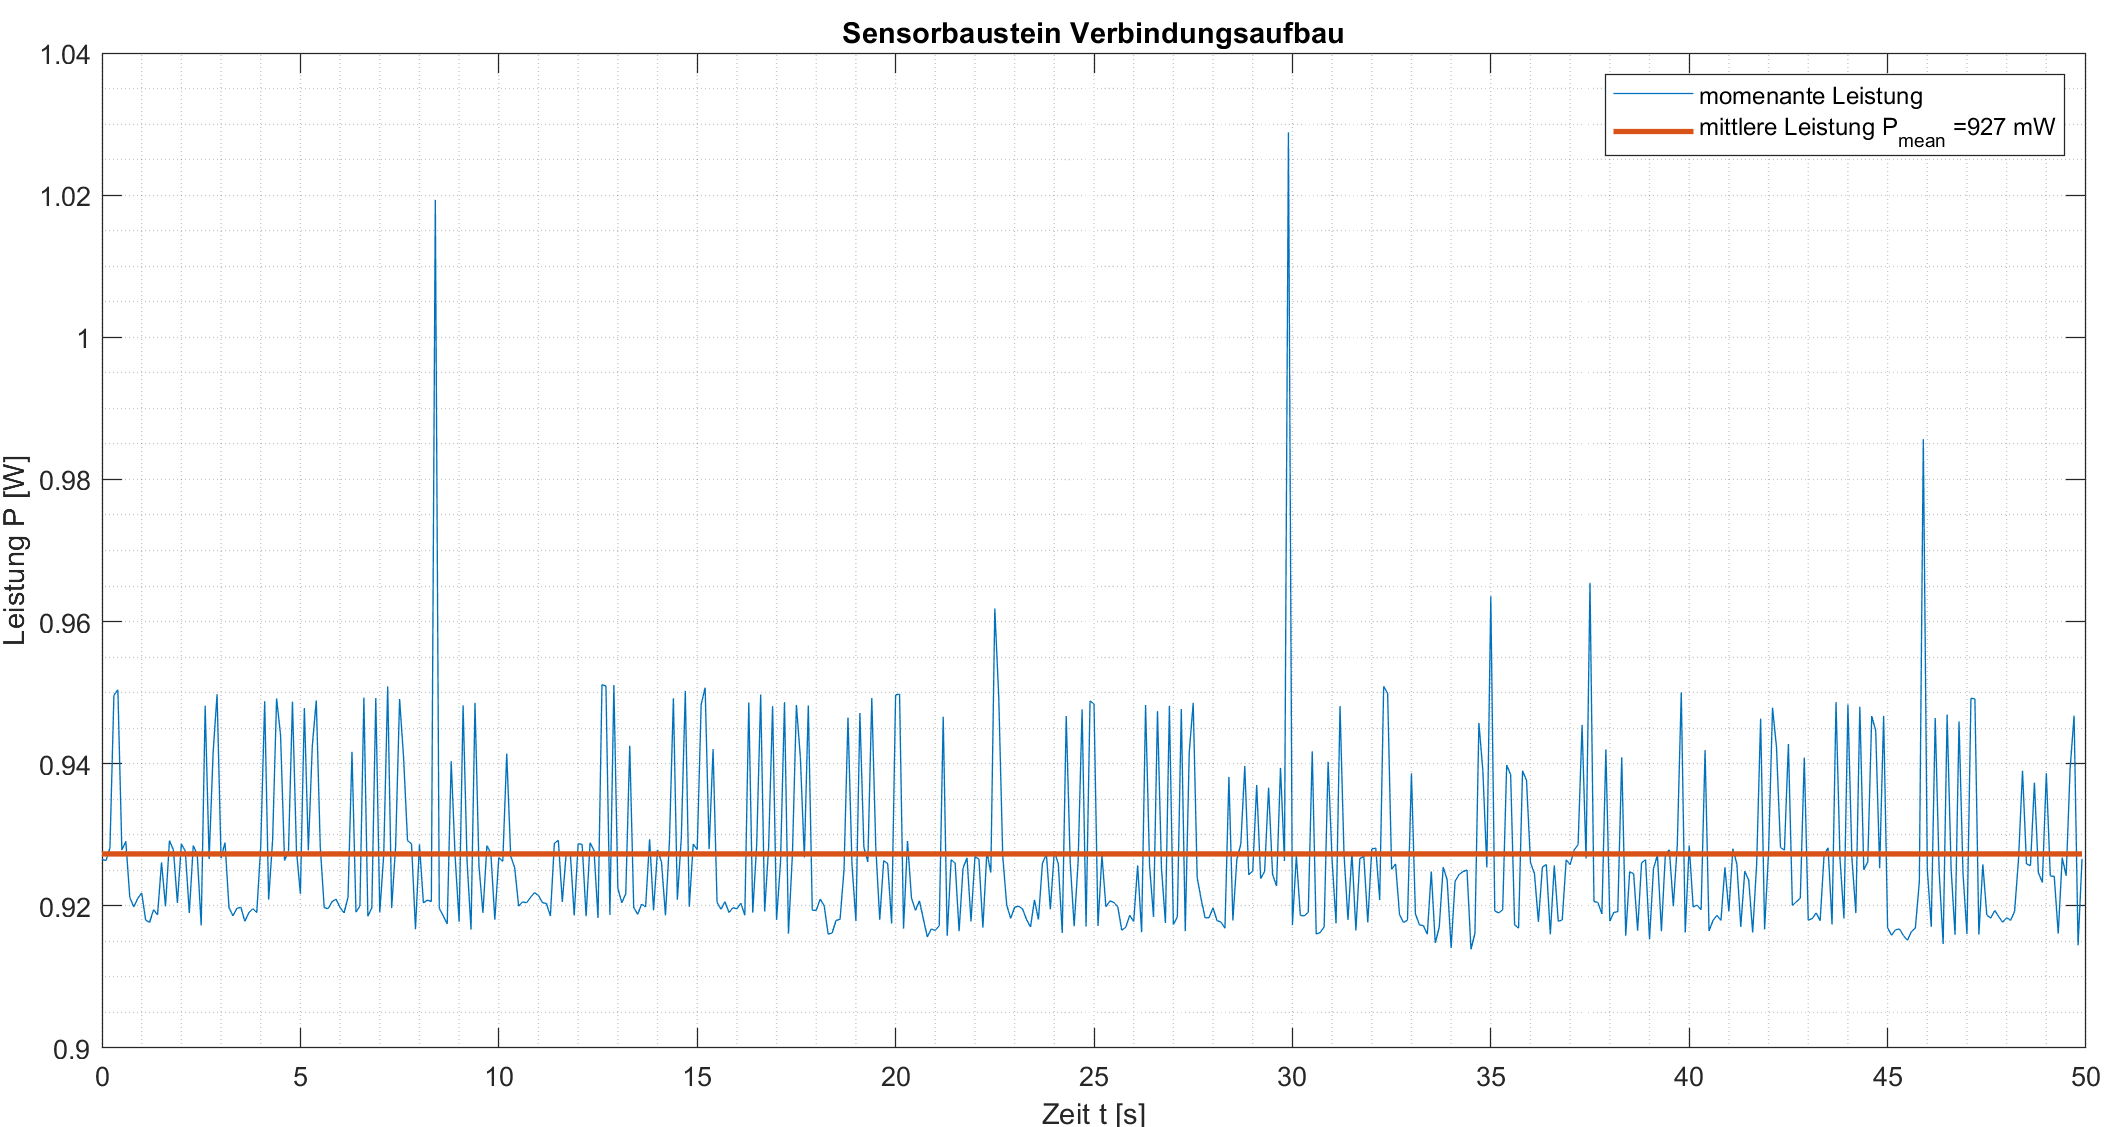
\includegraphics[width=1\textwidth]{graphics/Sensorbaustein_Verbindungsaufbau.png}
	\caption{Die Leistung des Sensorbausteins, wenn er einen Verbindungsaufbau versucht, aber kein geeignetes WLAN Netzwerk vorhanden ist}
	\label{pic: Sensorbaustein_verbindungsaufbau}
\end{figure}




\subsubsection{Temperatur}





